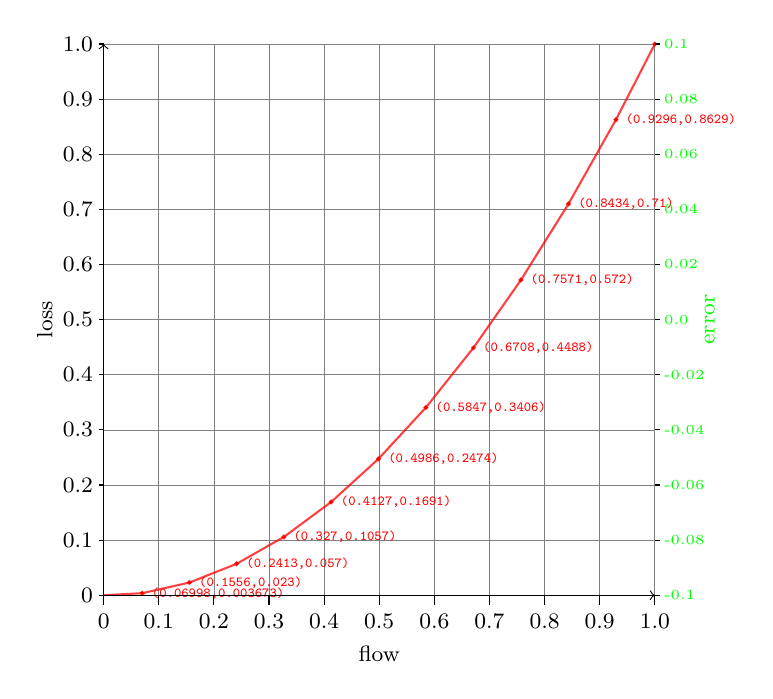
\begin{tikzpicture}[xscale=7.0,yscale=7.0]
\draw [help lines,step=0.1] (0,0) grid (1,1);
\draw[line width=0.5pt,color=black] plot file {default_12_XY.dat};
\coordinate (oneone) at (1,1);
\filldraw [red,draw opacity=0.75] (oneone) circle (0.1pt);
\coordinate (bk1) at (0,0);
\coordinate (bk2) at (0.069975,0.003673);
\coordinate (bk3) at (0.15564,0.023);
\coordinate (bk4) at (0.2413,0.057002);
\coordinate (bk5) at (0.32695,0.10568);
\coordinate (bk6) at (0.41274,0.16912);
\coordinate (bk7) at (0.49865,0.24742);
\coordinate (bk8) at (0.58467,0.34061);
\coordinate (bk9) at (0.67082,0.44876);
\coordinate (bk10) at (0.7571,0.57196);
\coordinate (bk11) at (0.84338,0.71004);
\coordinate (bk12) at (0.9296,0.86292);
\coordinate (bk13) at (1,1);
\filldraw [red,draw opacity=0.75] (bk2) circle (0.1pt) node[right] {\tiny \texttt{(0.06998,0.003673)}};
\filldraw [red,draw opacity=0.75] (bk3) circle (0.1pt) node[right] {\tiny \texttt{(0.1556,0.023)}};
\filldraw [red,draw opacity=0.75] (bk4) circle (0.1pt) node[right] {\tiny \texttt{(0.2413,0.057)}};
\filldraw [red,draw opacity=0.75] (bk5) circle (0.1pt) node[right] {\tiny \texttt{(0.327,0.1057)}};
\filldraw [red,draw opacity=0.75] (bk6) circle (0.1pt) node[right] {\tiny \texttt{(0.4127,0.1691)}};
\filldraw [red,draw opacity=0.75] (bk7) circle (0.1pt) node[right] {\tiny \texttt{(0.4986,0.2474)}};
\filldraw [red,draw opacity=0.75] (bk8) circle (0.1pt) node[right] {\tiny \texttt{(0.5847,0.3406)}};
\filldraw [red,draw opacity=0.75] (bk9) circle (0.1pt) node[right] {\tiny \texttt{(0.6708,0.4488)}};
\filldraw [red,draw opacity=0.75] (bk10) circle (0.1pt) node[right] {\tiny \texttt{(0.7571,0.572)}};
\filldraw [red,draw opacity=0.75] (bk11) circle (0.1pt) node[right] {\tiny \texttt{(0.8434,0.71)}};
\filldraw [red,draw opacity=0.75] (bk12) circle (0.1pt) node[right] {\tiny \texttt{(0.9296,0.8629)}};
\draw[line width=0.75pt,color=red,draw opacity=0.75] (bk1) -- (bk2); 
\draw[line width=0.75pt,color=red,draw opacity=0.75] (bk2) -- (bk3); 
\draw[line width=0.75pt,color=red,draw opacity=0.75] (bk3) -- (bk4); 
\draw[line width=0.75pt,color=red,draw opacity=0.75] (bk4) -- (bk5); 
\draw[line width=0.75pt,color=red,draw opacity=0.75] (bk5) -- (bk6); 
\draw[line width=0.75pt,color=red,draw opacity=0.75] (bk6) -- (bk7); 
\draw[line width=0.75pt,color=red,draw opacity=0.75] (bk7) -- (bk8); 
\draw[line width=0.75pt,color=red,draw opacity=0.75] (bk8) -- (bk9); 
\draw[line width=0.75pt,color=red,draw opacity=0.75] (bk9) -- (bk10); 
\draw[line width=0.75pt,color=red,draw opacity=0.75] (bk10) -- (bk11); 
\draw[line width=0.75pt,color=red,draw opacity=0.75] (bk11) -- (bk12); 
\draw[line width=0.75pt,color=red,draw opacity=0.75] (bk12) -- (bk13); 
\draw[->] (0,0) -- node[midway,yshift=-0.75cm] {\footnotesize flow} (1,0);
\draw[->] (0,0) -- node[rotate=90,midway,yshift=0.75cm] {\footnotesize loss} (0,1) ;
\foreach \x/\xtext in {0,0.1,0.2,0.3,0.4,0.5,0.6,0.7,0.8,0.9,1.0}
\draw (\x cm,0pt) -- (\x cm,-0.5pt) node[anchor=north] {\footnotesize \xtext};
\foreach \y/\ytext in {0,0.1,0.2,0.3,0.4,0.5,0.6,0.7,0.8,0.9,1.0}
\draw (0.0pt,\y cm) -- (-0.25pt,\y cm) node[anchor=east,xshift=0.5mm] {\footnotesize \ytext};
\draw[line width=0.5pt,color=green,draw opacity=0.75] plot file {default_12_err.dat};
\foreach \y/\ytext in {0/-0.1,0.1/-0.08,0.2/-0.06,0.3/-0.04,0.4/-0.02,0.5/0.0,0.6/0.02,0.7/0.04,0.8/0.06,0.9/0.08,1.0/0.1}
\draw (1cm,\y cm) -- (1.01cm,\y cm) node[anchor=west,xshift=-0.75mm] {\tiny \textcolor{green}{\ytext}};
\node[rotate=90] at (1.1,0.5) {\footnotesize \textcolor{green}{error}};
\end{tikzpicture}
